\documentclass{beamer}
% Remove navigation bar from the slide show.
\beamertemplatenavigationsymbolsempty

\usepackage{minted}
\usepackage{graphicx}

\usetheme{Malmoe}

\title{Why You Should Give Vim a Try}
\author{Mauri Mustonen (Kazhuu)}
\date{October 3, 2019 \\ TampereJS}

\definecolor{UniBlue}{RGB}{83,121,170}
\setbeamercolor{title}{fg=UniBlue}
\setbeamercolor{frametitle}{fg=UniBlue}
%\setbeamercolor{background canvas}{bg=gray}

\begin{document}
\maketitle

\usebackgroundtemplate{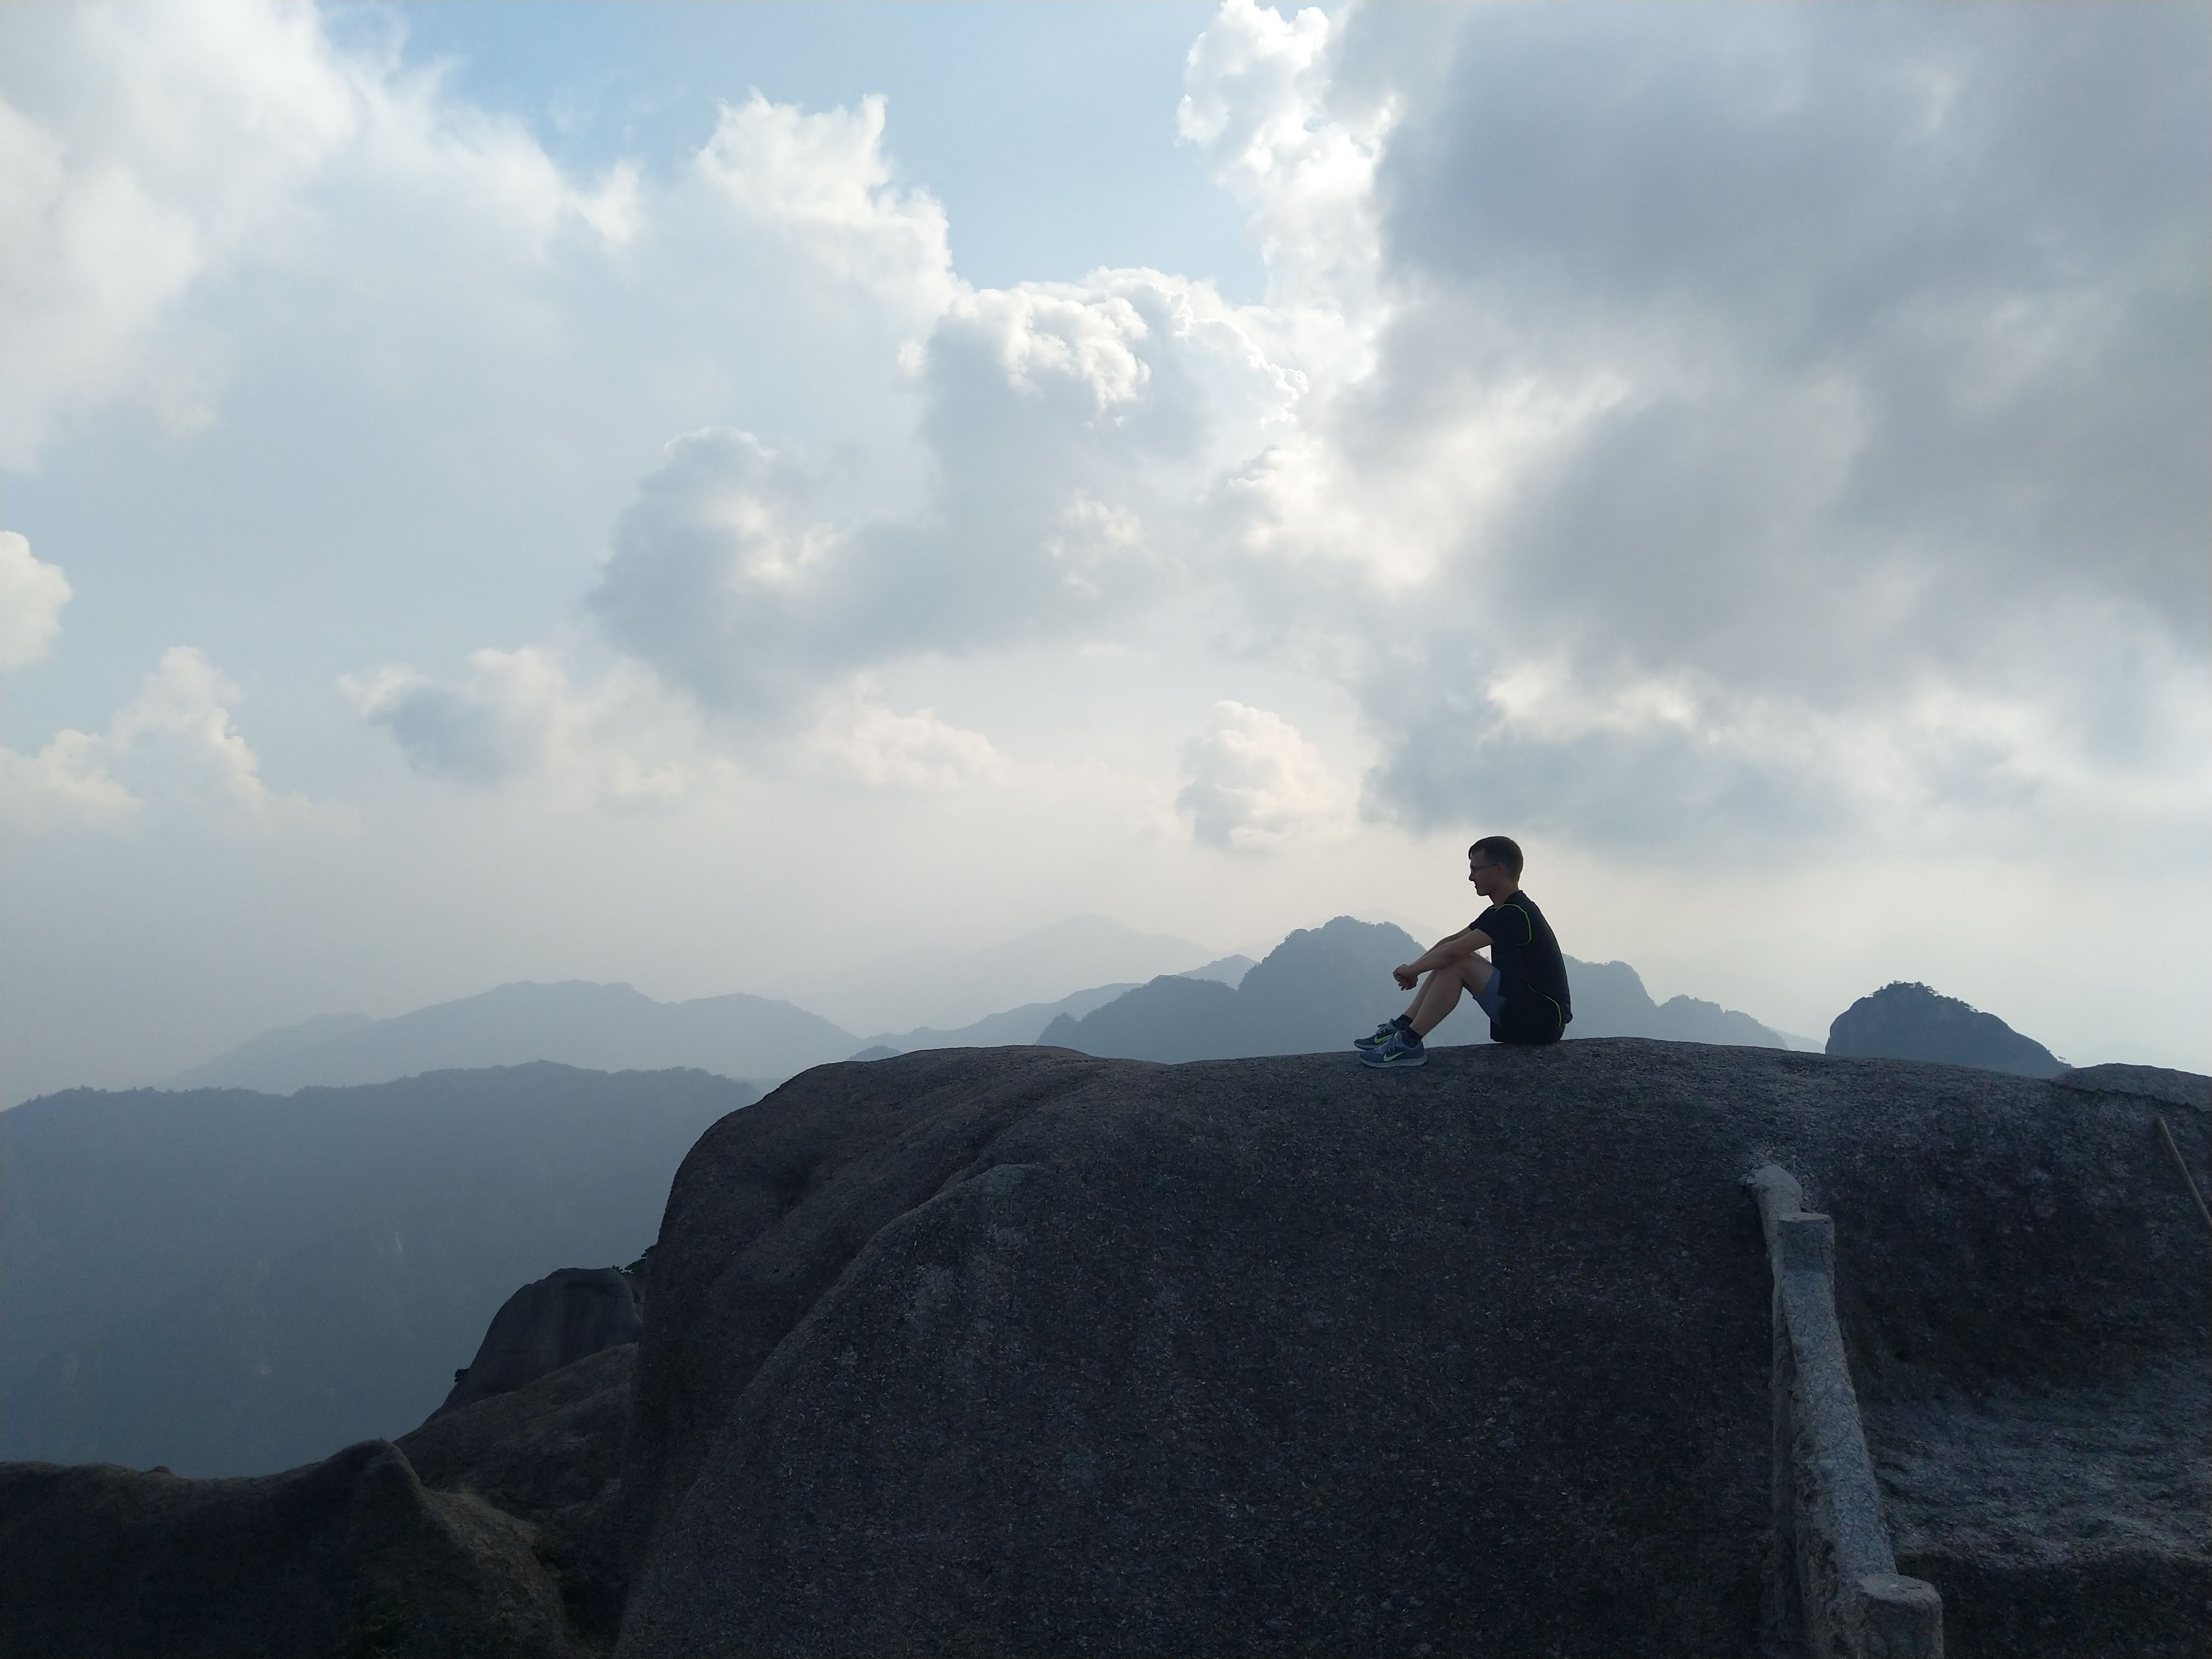
\includegraphics[width=\paperwidth,height=\paperheight]{images/me.jpg}}
\begin{frame}{Where To Find Me}
    \begin{itemize}
        \item Web page: \url{https://mauri.codes}
        \item GitHub: Kazhuu
        \item LinkedIn: Mauri Mustonen
    \end{itemize}
\end{frame}
\usebackgroundtemplate{}

\begin{frame}{Vim Learning Wall}
    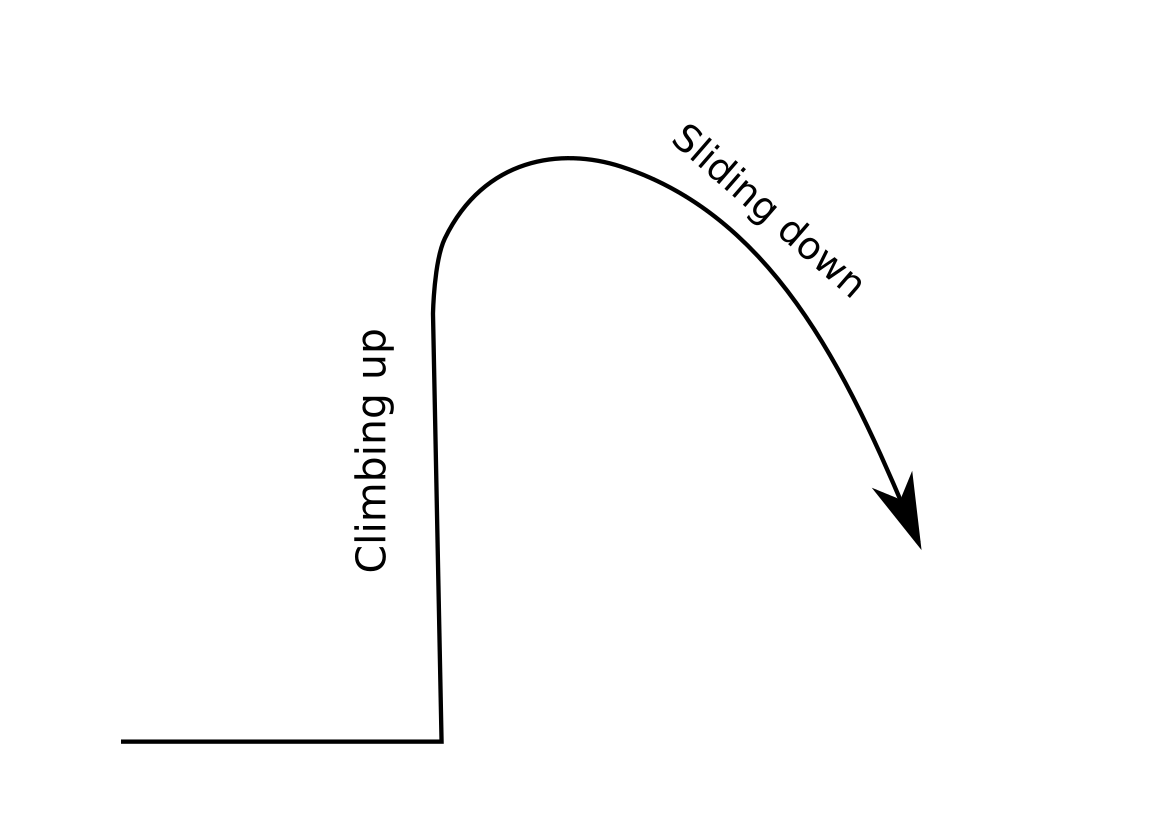
\includegraphics[width=1\textwidth]{images/vim-learning-curve.png}
\end{frame}

\usebackgroundtemplate{}
\begin{frame}{Why To Learn Vim}
    \begin{columns}
        \begin{column}{0.4\textwidth}
            \begin{center}
                
\includegraphics[width=1\textwidth]{images/vim-logo.png}
            \end{center}
        \end{column}
        \begin{column}{0.6\textwidth}
            \begin{itemize}
                \item Get rid of your mouse
                \item Less time on unnecessary hand movements
                \item Much more efficient code editing
                \item Highly customizable and extensible
                \item Learn new things for many years to come
                \item It will stick with you
                \item Become one of \textbf{those} people
            \end{itemize}
        \end{column}
    \end{columns}
\end{frame}

\begin{frame}{Vim Is All About Modes}
    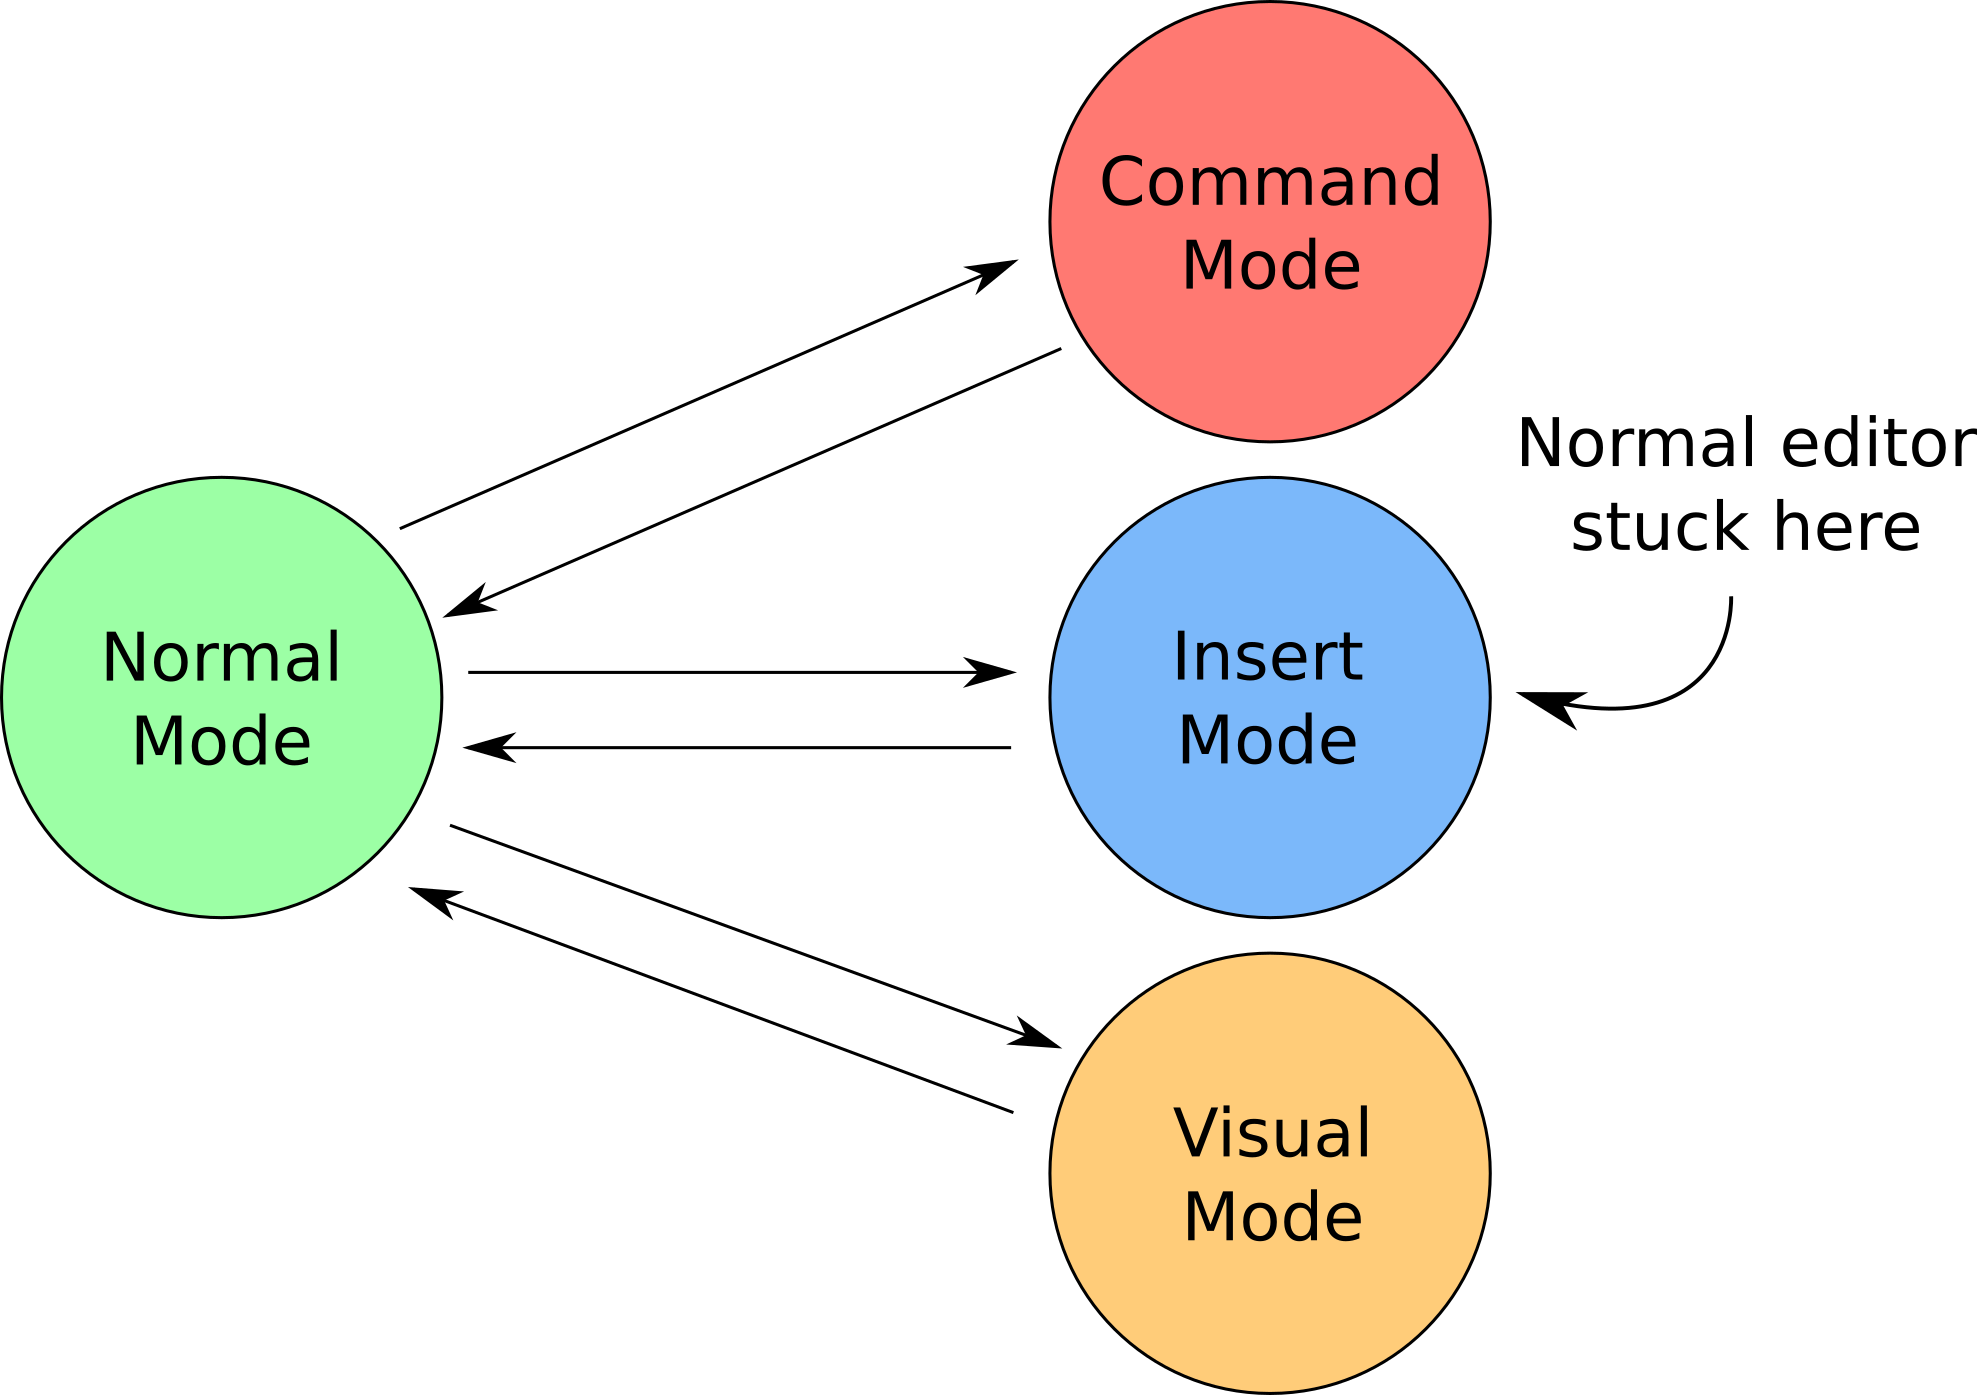
\includegraphics[width=1\textwidth]{images/vim-modes.png}
\end{frame}

\begin{frame}{Vim Is All About Modes}
    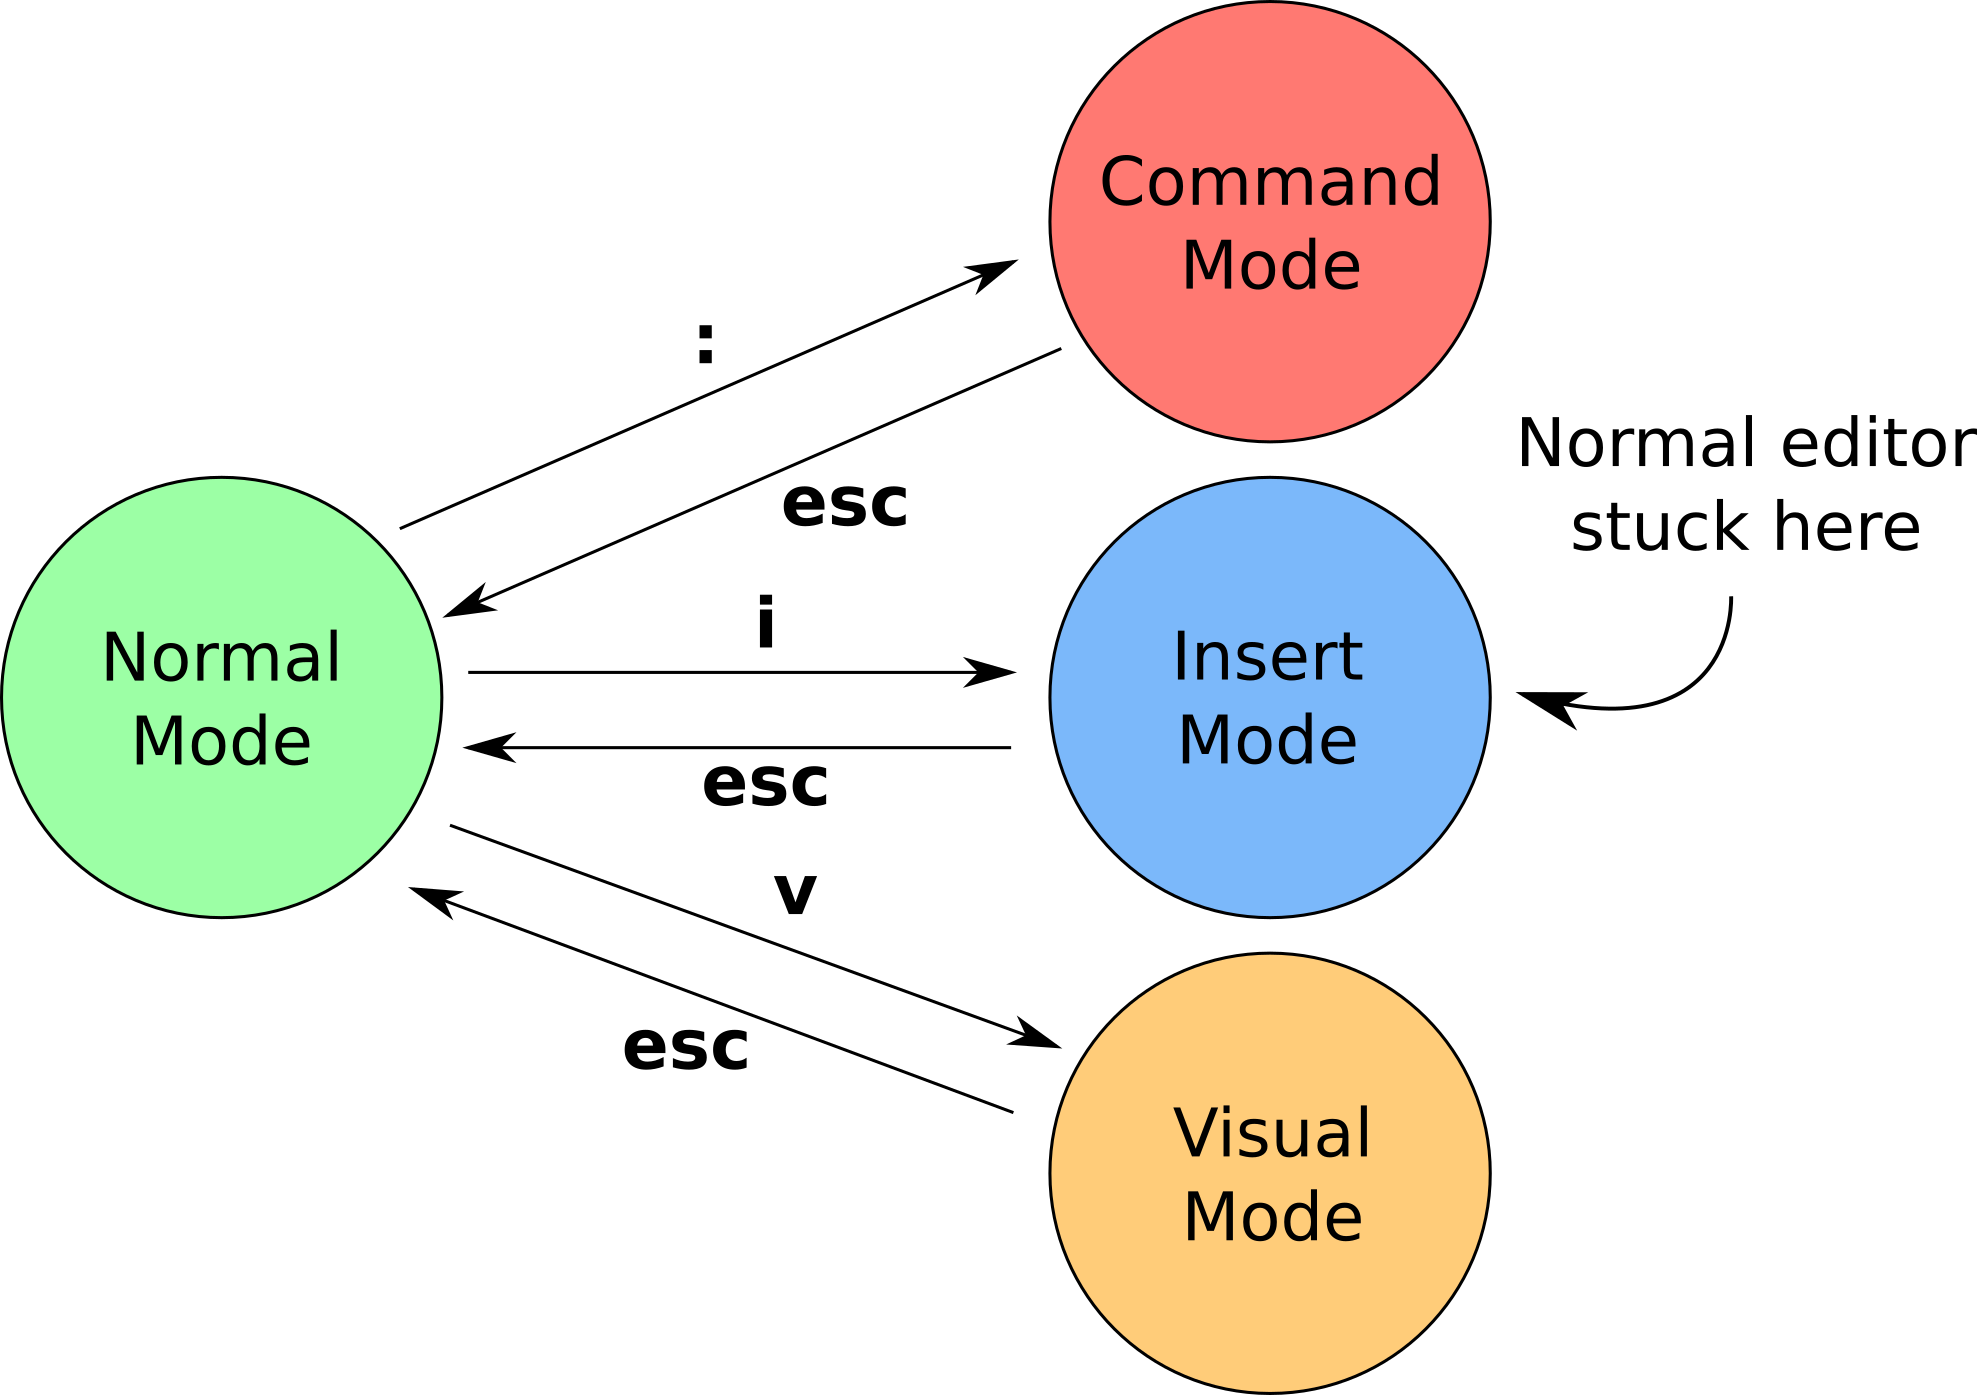
\includegraphics[width=1\textwidth]{images/vim-modes-keys.png}
\end{frame}

\begin{frame}{Basic Movement}
    \begin{columns}
        \begin{column}{0.2\textwidth}
            \begin{itemize}
                \item[--] \textbf{h}, \textbf{j}, \textbf{k}, \textbf{l}
                \item[--] \textbf{w}
                \item[--] \textbf{e}
                \item[--] \textbf{b}
                \item[--] \textbf{gg}
                \item[--] \textbf{G}
                \item[--] \textbf{0}
                \item[--] \textbf{\$}
            \end{itemize}
        \end{column}
        \begin{column}{0.8\textwidth}
            \begin{itemize}
                \item left, down, up, right
                \item move for\textbf{w}ard one word
                \item move forward to \textbf{e}nd of the word
                \item move \textbf{b}ackward one word
                \item move to the top of the file
                \item move to the bottom of the file
                \item move to the beginning of the line
                \item move to the end of the line
            \end{itemize}
        \end{column}
    \end{columns}
    \begin{center}
        \large And more...
    \end{center}
\end{frame}

\begin{frame}{Basic Editing}
    \begin{columns}
        \begin{column}{0.2\textwidth}
            \begin{itemize}
                \item[--] \textbf{i}
                \item[--] \textbf{d}
                \item[--] \textbf{c}
                \item[--] \textbf{y}
                \item[--] \textbf{p}
                \item[--] \textbf{u}
                \item[--] \textbf{ctrl+r}
                \item[--] \textbf{.}
            \end{itemize}
        \end{column}
        \begin{column}{0.8\textwidth}
            \begin{itemize}
                \item \textbf{i}nsert
                \item \textbf{d}elete
                \item \textbf{c}hange
                \item copy (\textbf{y}ank)
                \item \textbf{p}aste
                \item \textbf{u}ndo
                \item \textbf{r}edo
                \item repeat last command
            \end{itemize}
        \end{column}
    \end{columns}
    \begin{center}
        \large And more...
    \end{center}
\end{frame}

\begin{frame}{Composing Commands}
    \begin{center}
        \large \textless number\textgreater \textless command\textgreater
        \textless text object/motion\textgreater
    \end{center}
    \begin{columns}
        \begin{column}{0.2\textwidth}
            \begin{itemize}
                \item[--] \textbf{dw}
                \item[--] \textbf{yw}
                \item[--] \textbf{2dw}
                \item[--] \textbf{5j}
                \item[--] \textbf{dd}
                \item[--] \textbf{50G}
            \end{itemize}
        \end{column}
        \begin{column}{0.5\textwidth}
            \begin{itemize}
                \item \textbf{d}elete next \textbf{w}ord
                \item copy/\textbf{y}ank \textbf{w}ord
                \item \textbf{d}elete two following \textbf{w}ords
                \item move down five lines
                \item delete line
                \item go to line 50
            \end{itemize}
        \end{column}
    \end{columns}
\end{frame}

\begin{frame}{Command Language}
    \begin{block}{How to delete all function parameters?}
    \end{block}
    \inputminted{js}{codes/changeInsideParentheses.js}
    \pause
    \begin{center}
        \huge
        ci)
        \\
        \textbf{c}hange \textbf{i}nside \textbf{p}arentheses
    \end{center}
\end{frame}

\begin{frame}{Command Language}
    \begin{block}{How to change string inside quotes?}
    \end{block}
    \inputminted{js}{codes/changeInsideQuotes.js}
    \pause
    \begin{center}
        \huge
        ci'
        \\
        \textbf{c}hange \textbf{i}nside \textbf{q}uotes
    \end{center}
\end{frame}

\begin{frame}{Command Language}
    \begin{block}{How to rewrite the whole function body?}
    \end{block}
    \inputminted{js}{codes/changeInsideBlock.js}
    \pause
    \begin{center}
        \huge
        ci\}
        \\
        \textbf{c}hange \textbf{i}nside \textbf{b}races
    \end{center}
\end{frame}

\begin{frame}{Configuring .vimrc}
    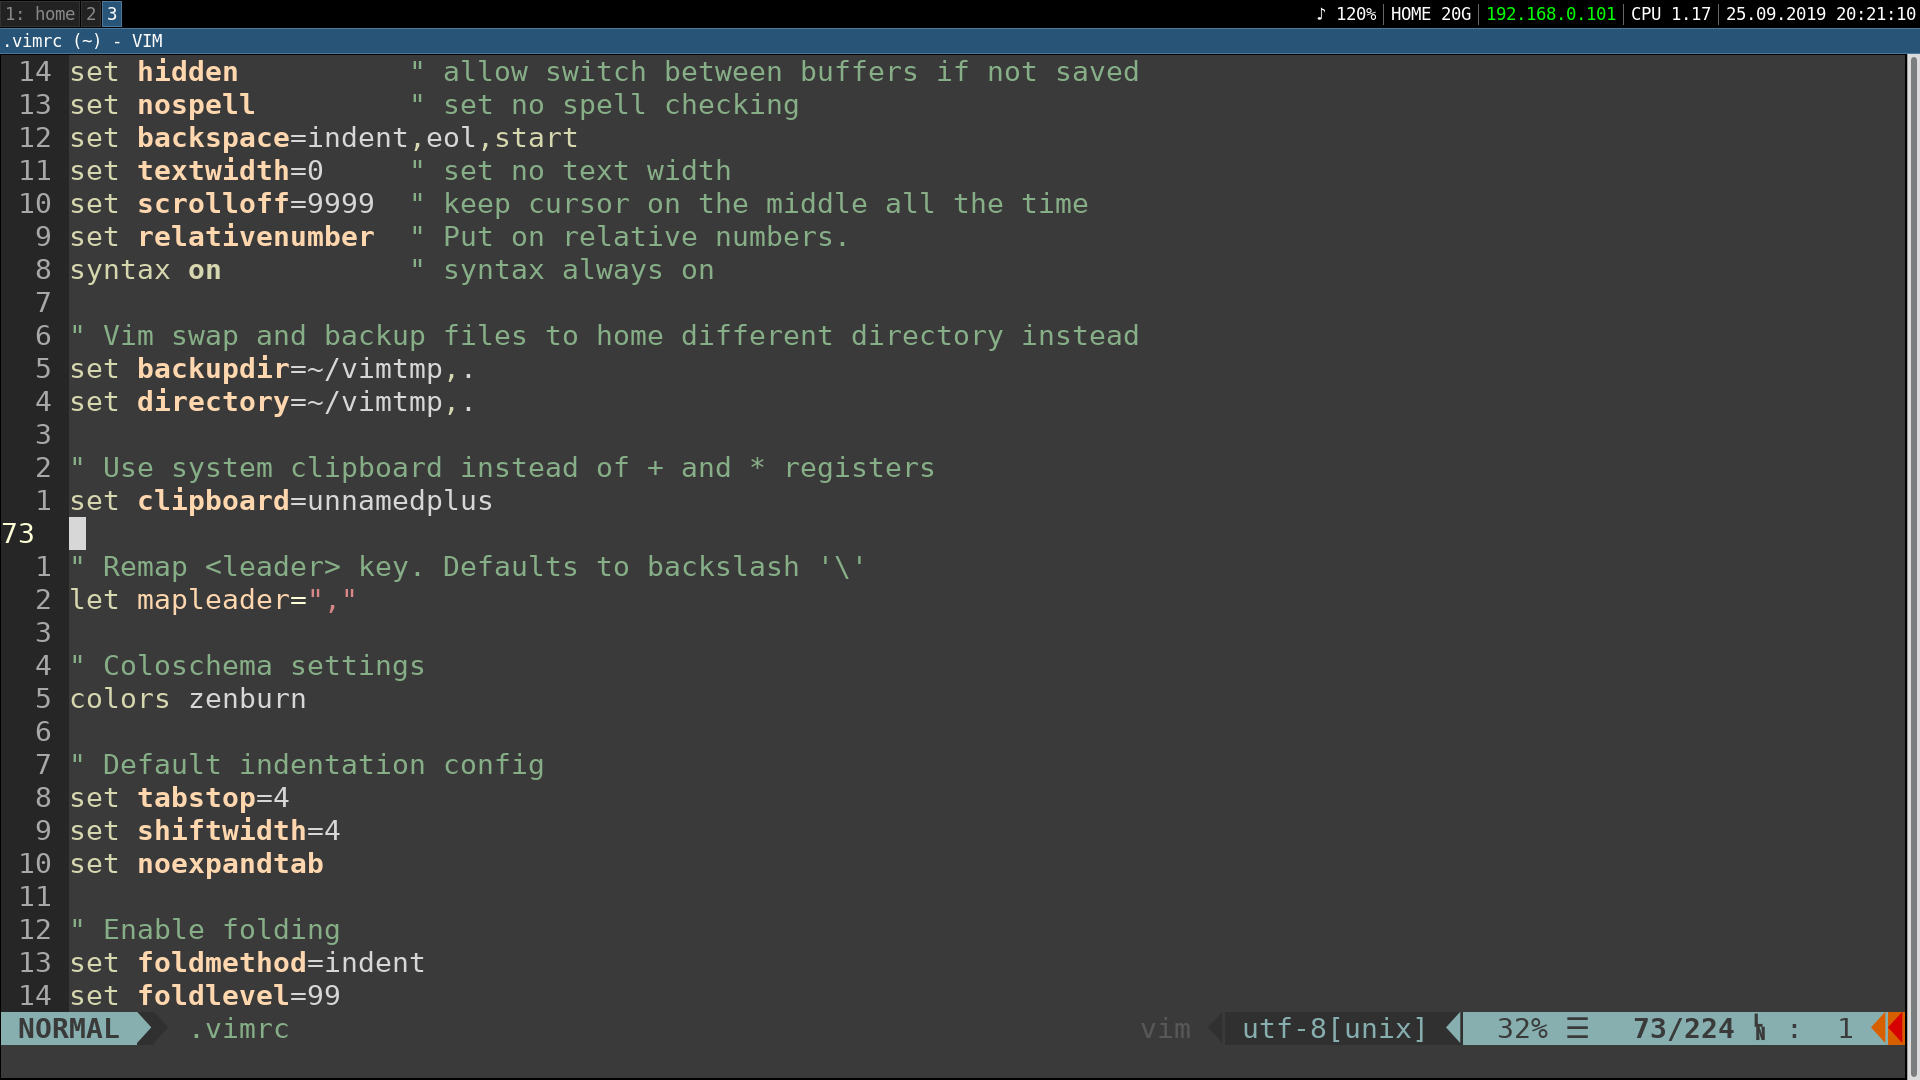
\includegraphics[width=1\textwidth]{images/vimrc.png}
\end{frame}

\begin{frame}{Some Useful Plugins}
    \begin{itemize}
        \item NERDTree
        \item Command-line fuzzy finder (fzf)
        \item Silver Searcher (ag)
        \item YouCompleteMe
    \end{itemize}
\end{frame}

\begin{frame}{Useful Tips}
    \begin{itemize}
        \item Escape to Caps Lock
        \item Tabs as \textbf{views}
        \item Registers as multiple clipboards
        \item Record macros
        \item Repeat with .
        \item Own cheat sheet
        \item Get help with :help
    \end{itemize}
\end{frame}

\begin{frame}{Vimtutor}
    \begin{center}
        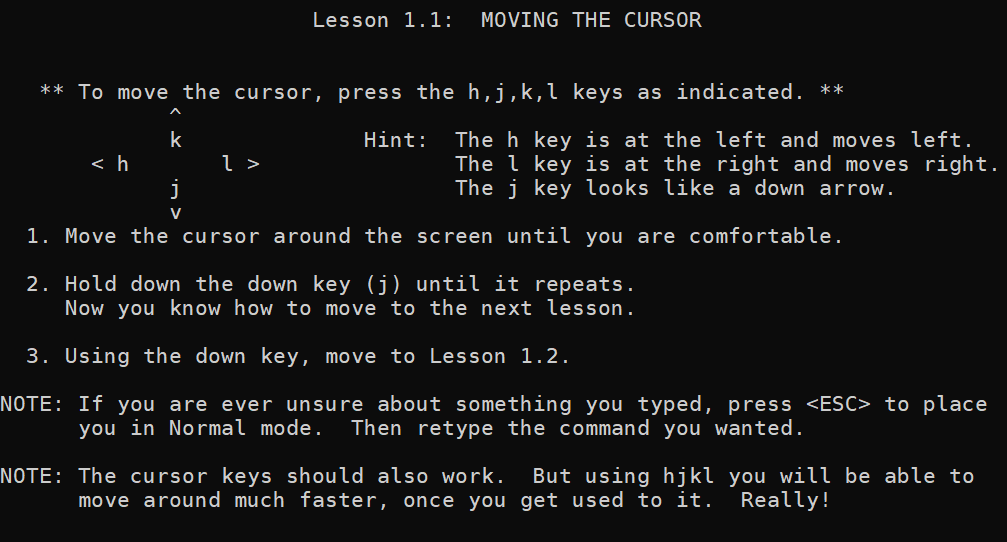
\includegraphics[width=1\textwidth]{images/vimtutor.png}
    \end{center}
\end{frame}

\begin{frame}{Vim Adventures}
    \begin{center}
        
\includegraphics[width=1\textwidth]{images/vim-adventure.png}
    \end{center}
\end{frame}

\begin{frame}
    \begin{center}
        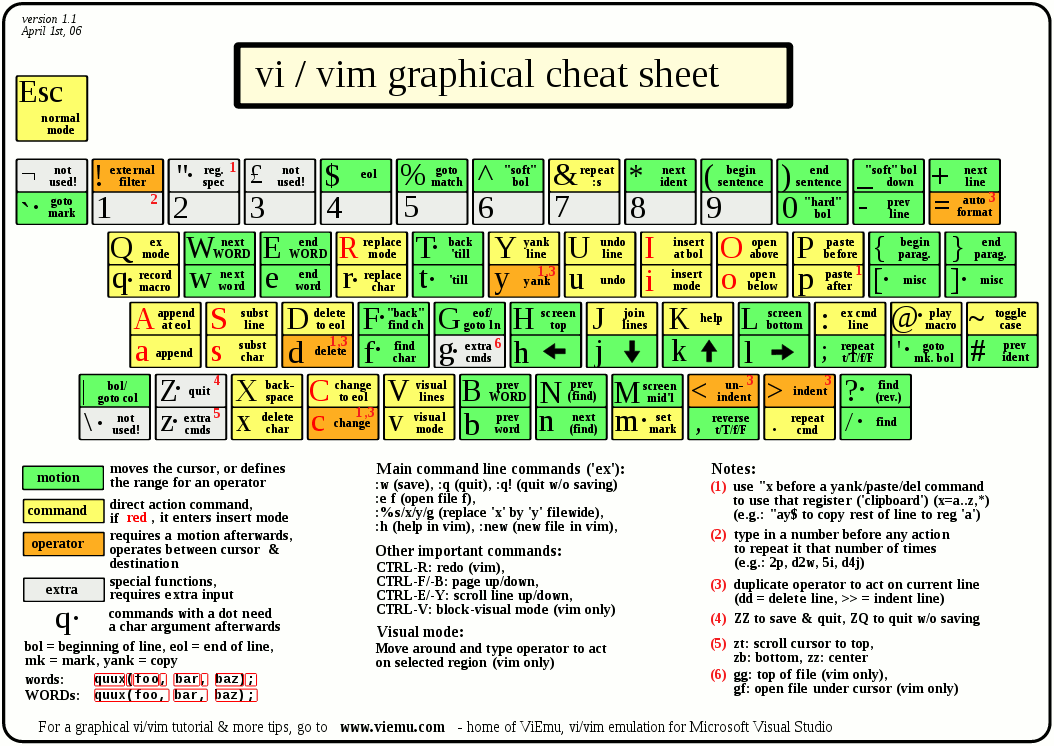
\includegraphics[width=1\textwidth]{images/cheat-sheet.png}
    \end{center}
\end{frame}

\begin{frame}{Vim Elsewhere}
    \begin{columns}
        \begin{column}{0.4\textwidth}
            \begin{center}
                
\includegraphics[width=1\textwidth]{images/i3wm-logo.png}
            \end{center}
        \end{column}
        \begin{column}{0.6\textwidth}
            \begin{itemize}
                \item Chrome with Vimium
                \item Linux i3 window manager
                \item Vim on Windows Subsystem for Linux (WSL)
            \end{itemize}
        \end{column}
    \end{columns}
\end{frame}

\begin{frame}{Summary}
    \begin{itemize}
        \item Vim is hard because it's different
        \item Start with basics
        \item Make your own .vimrc and understand it
        \item Read other people's .vimrc files
        \item Make your own cheat sheet
        \item Take time and learn
        \item You will become much more efficient editing code
        \item Highly customizable and extensible
    \end{itemize}
\end{frame}

\begin{frame}
    \begin{center}
        \huge Thank you for your time!
    \end{center}
    \begin{center}
        \large Questions?
    \end{center}
    \begin{center}
        https://mauri.codes
    \end{center}
\end{frame}
\end{document}
